\documentclass[11pt]{article}
\usepackage[T1]{fontenc}
\usepackage{lmodern,microtype,geometry,amsmath,amssymb,booktabs,graphicx,tabularx,longtable,float,xcolor}
\usepackage[colorlinks=true,linkcolor=teal,citecolor=teal,urlcolor=teal]{hyperref}
\geometry{margin=0.85in}
\setlength{\parskip}{0.35em}\setlength{\parindent}{0pt}
\graphicspath{{../results/figures/}}
\newcommand{\RpairC}{0}
\newcommand{\RfullC}{0.208806}
\newcommand{\RvertexD}{0.178834}
\newcommand{\RexactD}{0.3}
\newcommand{\RadiusA}{0.1}
\newcommand{\ExitA}{1.5}
\newcommand{\DetectSixteen}{43}
\newcommand{\DetectOneTwoEight}{97}

\title{TAFR-Knee: Exact Mechanism Checks,\newline Benchmark Pilots, and an Article Outline}
\author{Research note for the TAFR-Knee project}\date{6 September 2026}
\begin{document}\maketitle
\begin{abstract}
Finite-radius knee claims require separate geometry, optimizer-map, and gain checks.
We implement a linear-programming oracle that identifies objective vectors reachable under bounded weight perturbations in a finite table.
The oracle establishes counterexamples to pairwise perturbations and vertex-only auditing, while an absolute-gain test exposes a ratio-based screening failure.
Versioned experiments connect these mechanisms to the sensitivity knee (SNEE) approach, the PMOP knee benchmark suite, enumerated project portfolios, and two ammonia scheduling windows.
The evidence supports the audit framework and identifies conditions that a final algorithm must address.
The benchmark comparisons remain pilots; they do not establish general superiority or a continuous global certificate.
\end{abstract}

\section{Preference stability needs separate checks}
Decision makers need compromises whose objective values remain acceptable when preferences change.
A stable optimizer output can nevertheless be an extreme solution, and a sampled audit can miss a reachable optimizer response.
TAFR-Knee, short for Trade-off-Active Finite-Radius Knee Detection, separates these concerns through normalization, preference perturbations, anchor-distance screening, and exit trade-offs.
This note tests that separation before proposing final empirical claims.

The 2024 Thesis Proposal Exam (TPE) proposal introduced a weight-perturbation min--max formulation and a Karush--Kuhn--Tucker reformulation~\cite{proposal}.
We preserve that starting point through a TPE-2024-grid reconstruction that minimizes raw squared objective displacement under pairwise perturbations.
Its finite candidate search does not reproduce the proposal's full constrained reformulation.
The production TAFR core remains unchanged at commit \texttt{9f7a65d7}.
The TAFR gain variant raises both absolute exit-gain thresholds to $10^{-3}$ through the existing configuration interface.

The note contributes an exact finite-table oracle, mechanism-specific evidence, and a versioned pilot record.
Sections~\ref{sec:oracle} and~\ref{sec:mechanisms} define the oracle and explain the counterexamples.
Sections~\ref{sec:snee} through~\ref{sec:ammonia} report completed comparisons and their limits.
Section~\ref{sec:outline} turns those findings into an article outline and remaining experimental gates.


Table~\ref{tab:roles} compares method inputs and analyses. Here RI denotes robustness index and AWT denotes augmented weighted Tchebycheff scalarization.
\begin{table}[htbp]\centering\small
\begin{tabularx}{\linewidth}{l*{4}{>{\raggedright\arraybackslash}X}}
\toprule
Method & Selection input & Derivatives & Finite weight analysis & Discrete models \\
\midrule
TAFR & Candidate weights & Solver dependent & Sampled severity; external exact table oracle & Via callback \\
SNEE & Scalarized problems & First and second order & Local sensitivity & Outside published smooth assumptions \\
Mavrotas RI & Selected Pareto point & Solver dependent & Sampled persistence & Yes, including AWT \\
Post-hoc geometric rules & Front approximation & Usually no & Usually absent & Through supplied front \\
\bottomrule
\end{tabularx}
\caption{Conceptual roles differ across comparison families~\cite{snee,mavrotas,pmop}. No row asserts equal implementation maturity in this release.}\label{tab:roles}
\end{table}

\section{The oracle checks reachable outputs}\label{sec:oracle}
Let $F(x)\in\mathbb R^m$ contain objectives that we minimize, and let $w$ belong to the probability simplex $\Delta_m$.
Frozen ideal and reference vectors $z,r$ define
\[
 \widetilde F_i(x)=\frac{F_i(x)-z_i}{r_i-z_i},\quad r_i>z_i,\qquad
 \mathcal U_\rho(w_0)=\{w\in\Delta_m:|w_i-w_{0i}|\le\rho\}.
\]
The weighted-sum solver minimizes $w^\top\widetilde F(x)$, equivalently using physical coefficients $w_i/(r_i-z_i)$.
Its finite-radius displacement is
\[
 R_\rho=\sup_{w\in\mathcal U_\rho(w_0)}
 \|\widetilde F(x(w))-\widetilde F(x(w_0))\|_2.
\]
Displacement measures worst-case severity; the probability of retaining a solution measures a different property.

For each normalized finite-table row $y^s$, a linear program intersects its weighted-sum optimality cell with the neighborhood:
\[
 w^\top(y^s-y^t)\le0\quad\forall t,\quad \mathbf1^\top w=1,\quad
 \max(0,w_0-\rho)\le w\le\min(1,w_0+\rho).
\]
The implementation uses a canonical lexicographic objective order for ties.
For higher-priority competitors, it maximizes a common strict margin and rejects rows reachable only through losing boundary ties.
The largest distance among reachable rows gives the deterministic table solver's $R_\rho$, subject to linear-programming feasibility tolerance $10^{-9}$.

The stability oracle minimizes the $L_\infty$ distance from $w_0$ to each reachable competing cell's closure.
It includes every competitor's inequalities: tying the nominal row alone need not make another row optimal.
An objective tolerance $\epsilon$ excludes competitors with displacement at most $\epsilon$.
The returned radius is a supremum; the deterministic tie rule determines whether the boundary itself retains the nominal solution.
Exhaustive two- and three-objective grid tests agree with the oracle on the supplied parity cases.

The production field \texttt{certified} has narrower semantics than a global mathematical certificate.
It checks distance from fitted anchors and an active exit ratio, then ranks accepted candidates by reported displacement and stability radius.
The screening predicate does not require $R_\rho\le\epsilon$.
We therefore call a returned pilot point ``screen-passed'' and reserve ``exact'' for finite-table oracle results.
Continuous validation with independent samples gives a lower bound on the true maximum.

\section{Counterexamples separate the mechanisms}\label{sec:mechanisms}
\subsection{Stable plateaus can include anchors}
The table $A=(0,10)$, $K=(4,4)$, $B=(10,0)$ separates plateau stability from compromise quality.
Scalarized costs give $K$ the co-optimality interval $w_1\in[0.4,0.6]$.
At equal weights, the exact stability radius is $\RadiusA$; a normalized exit to either anchor has improvement $0.4$, deterioration $0.6$, and ratio $\ExitA$.
The proposal reconstruction selects an anchor through its risk tie-break, while full TAFR selects $K$.
Removing only the non-extreme screen also selects $K$: the remaining exit rule rejects the anchors, so this case does not independently prove the necessity of that single screen.
\begin{figure}[htbp]\centering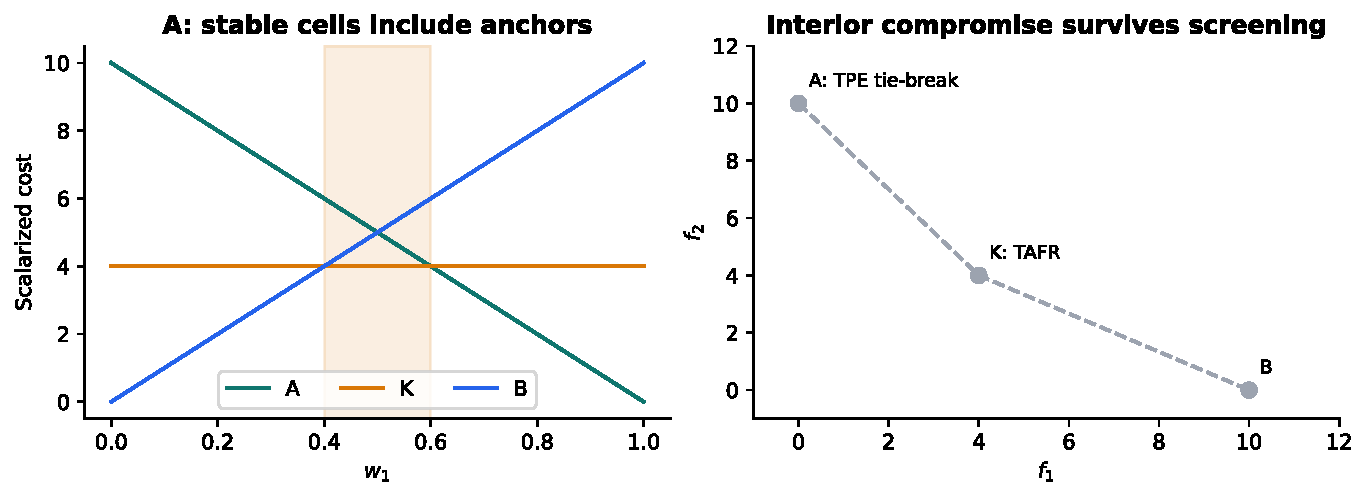
\includegraphics[width=0.95\linewidth]{case_A.pdf}
\caption{Plateau stability alone does not identify the interior compromise.}\end{figure}

Multiplying the second objective by $c\in\{1,10,100,1000,10000\}$ moves the raw-weight knee interval to
\[
 \left[\frac{4c}{6+4c},\frac{6c}{4+6c}\right].
\]
Frozen normalization preserves the selected normalized point within $10^{-8}$ across all five tables.
The unnormalized variant can abstain when its grid misses the narrow interval.
Figure~\ref{fig:B} separates abstention from selection error.
Scale invariance presumes valid bounds; Section~\ref{sec:pmop} tests the anchor estimator itself.
\begin{figure}[htbp]\centering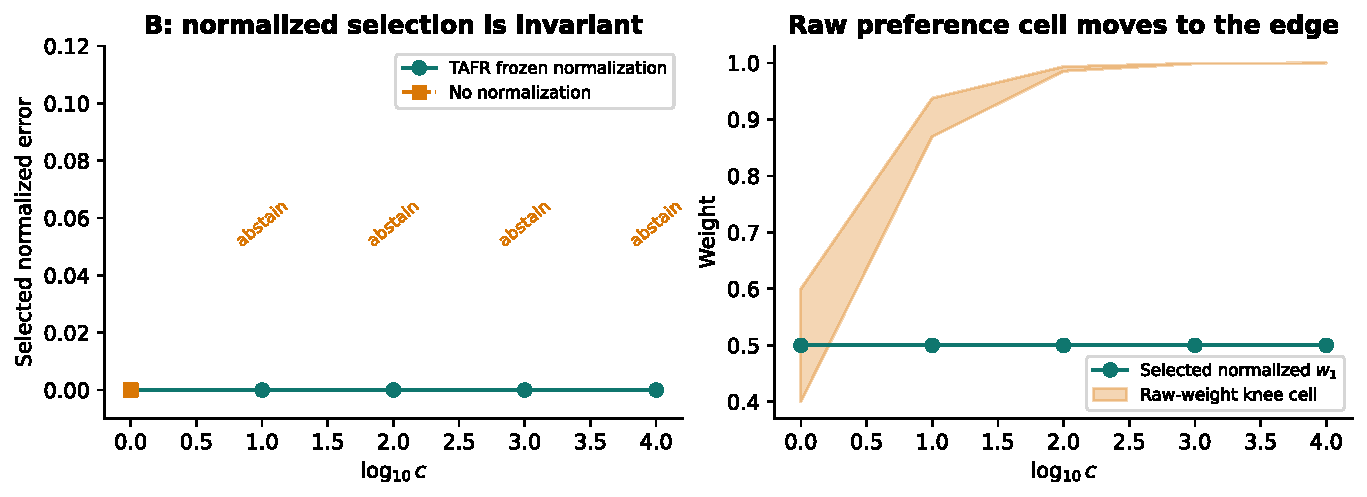
\includegraphics[width=0.95\linewidth]{case_B.pdf}
\caption{Normalization preserves selected geometry under objective rescaling.}\label{fig:B}\end{figure}

\subsection{Vertices repair only weight geometry}
Four objectives admit group perturbations that pairwise transfers omit.
For four anchors with zero diagonal and ten elsewhere, add $P=(5,5,5,5)$ and $Q=(4.3,4.3,6.3,6.3)$.
At $w_0=(1/4,1/4,1/4,1/4)$ and $\rho=0.1$, every pairwise transfer retains $P$.
Figure~\ref{fig:C} uses red for $+0.1$, blue for $-0.1$, and gray for zero. The perturbation $\delta=(0.1,0.1,-0.1,-0.1)$ gives the feasible weight $w_0+\delta=(0.35,0.35,0.15,0.15)$, which selects $Q$.
Pairwise auditing reports $\RpairC$; complete vertices and the oracle agree at $\RfullC$.
\begin{figure}[htbp]\centering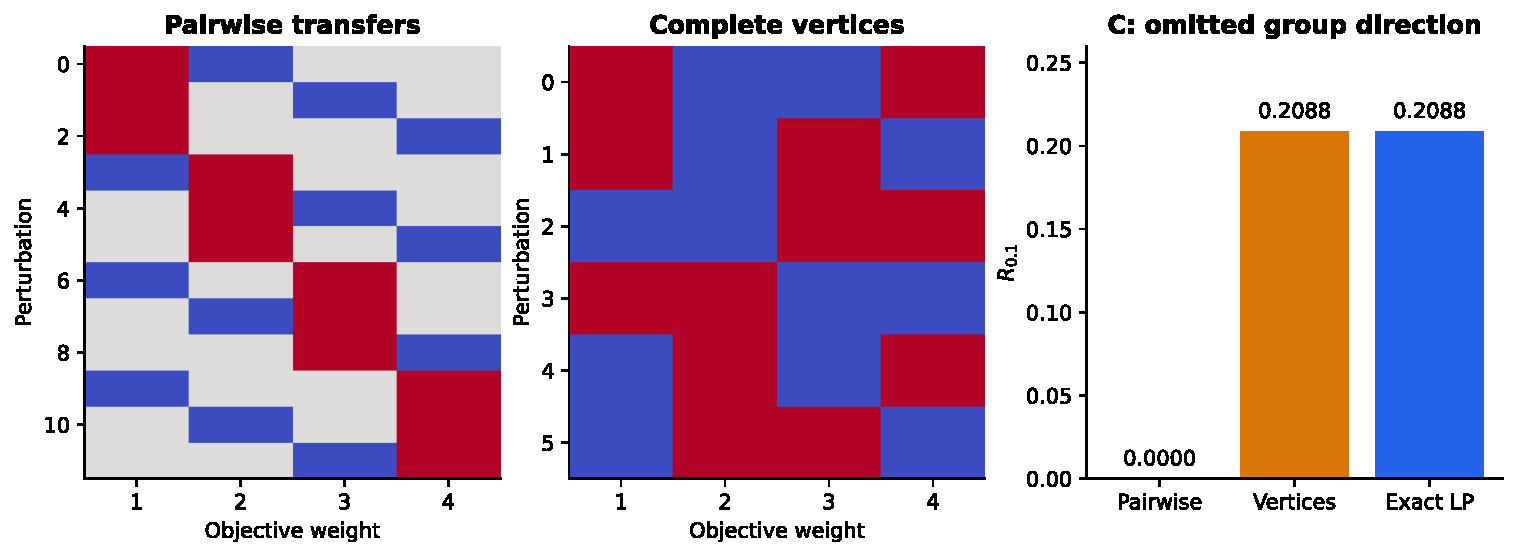
\includegraphics[width=\linewidth]{case_C.pdf}
\caption{A simultaneous two-up, two-down perturbation reveals the missed switch.}\label{fig:C}\end{figure}

Complete weight vertices need not maximize displacement through an optimizer map.
The seven-row three-objective case contains anchors, $P=(3,3,3)$, $Q=(1,4,5)$, and two shielding rows $R_1=(2.3426,3.6574,3.0600)$ and $R_2=(2.1564,2.4325,4.4712)$.
At $w_0=(1/3,1/3,1/3)$ and $\rho=0.18$, vertex-only auditing reports $\RvertexD$; the exact value is $\RexactD$.
The interior weight $(0.48,0.26,0.26)$ selects $Q$, while every neighborhood vertex selects another row.
Figure~\ref{fig:Dcells} displays the missed optimizer cell.
\begin{figure}[htbp]\centering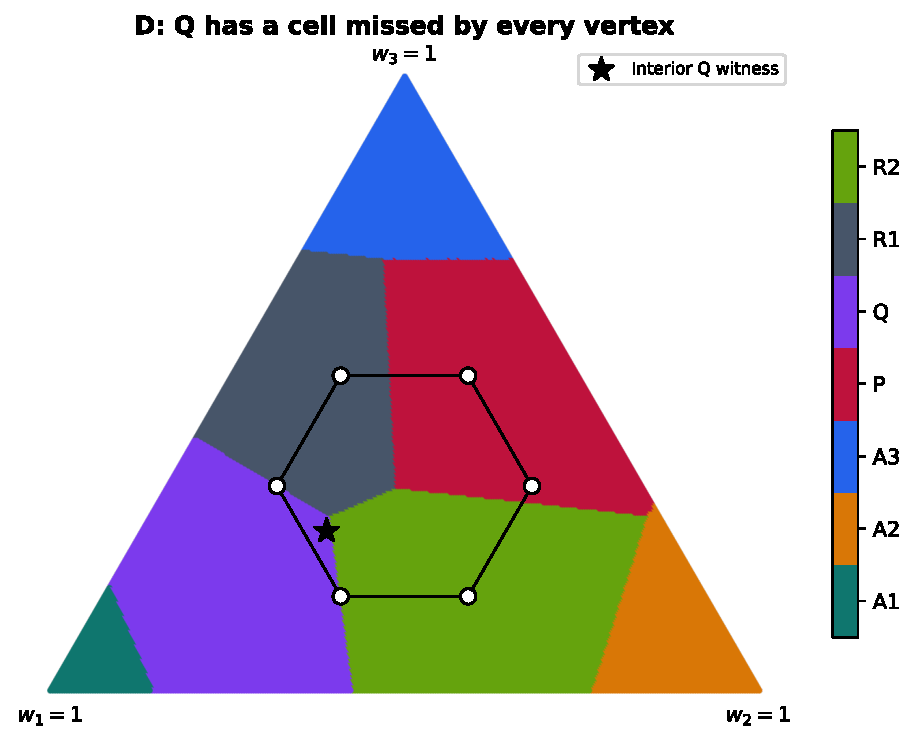
\includegraphics[width=0.60\linewidth]{case_D_cells.pdf}
\caption{The cell of $Q$ intersects the neighborhood away from every vertex.}\label{fig:Dcells}\end{figure}

Interior sampling improves detection without establishing a global bound.
Across 100 seeds, 16 samples detect the exact worst-case row in $\DetectSixteen$ runs, and 128 samples detect it in $\DetectOneTwoEight$ runs.
Hybrid auditing combines complete vertices, pairwise transfers, and hit-and-run interior samples. Adaptive rounds add hit-and-run samples starting from the worst output found so far.
Figure~\ref{fig:Ddetect} reports Wilson 95\% intervals and audit gap against solver calls.
Let $Y$ contain the seven objective rows of this example. A strictly convex quadratic companion uses $p\in\Delta_7$ and objectives $Y_{\cdot i}^\top p+(\tau/2)\|p\|_2^2$ for $\tau\in\{10^{-3},10^{-2}\}$.
Its interior witness also exceeds its vertex displacement, but that witness is not an exact continuous maximum.
The limitation therefore extends beyond discontinuous table selection.
\begin{figure}[htbp]\centering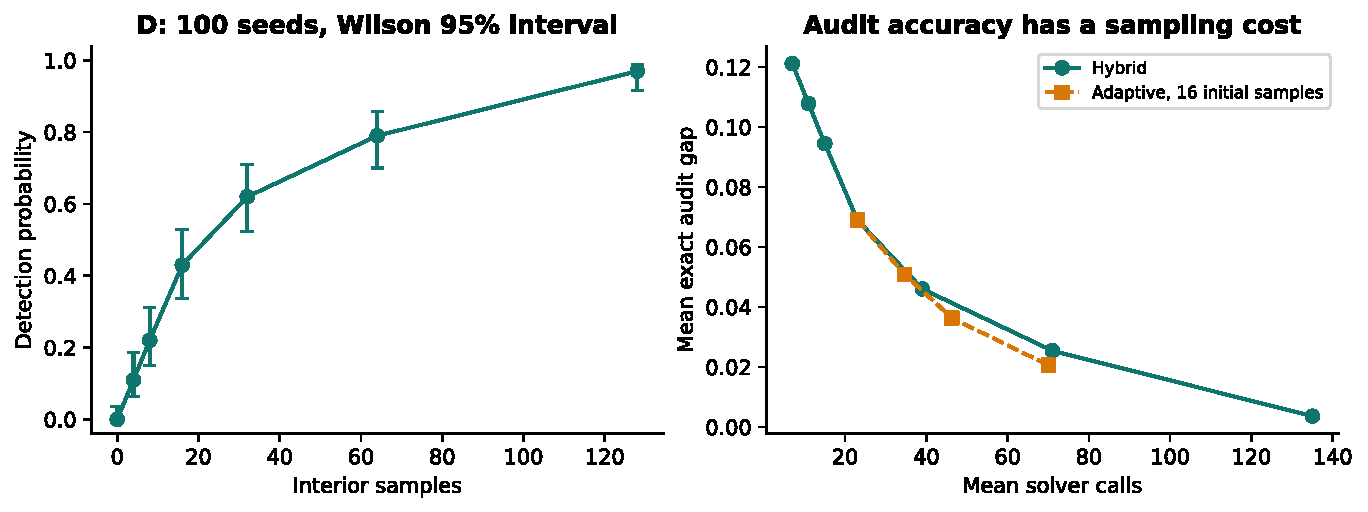
\includegraphics[width=0.96\linewidth]{case_D_detection.pdf}
\caption{Sampling reduces the gap, with residual misses even at 128 samples.}\label{fig:Ddetect}\end{figure}

\subsection{Absolute gains constrain exit ratios}
An exit ratio can grow while the decision improvement vanishes.
For nominal point $(0.5,0.5,0.5)$ and exit $(0.5-\eta,0.9,0.5)$, total improvement is $I=\eta$, total deterioration is $D=0.4$, and $K_{\rm exit}=D/I$.
The default activity rule accepts $\eta=10^{-5}$; its large ratio primarily reflects a small denominator.
The TAFR gain variant requires $I,D\ge10^{-3}$; Figure~\ref{fig:E} also sweeps $10^{-4}$, $5\times10^{-3}$, and $10^{-2}$.
We retain the production default and report absolute gains alongside the ratio.
\begin{figure}[htbp]\centering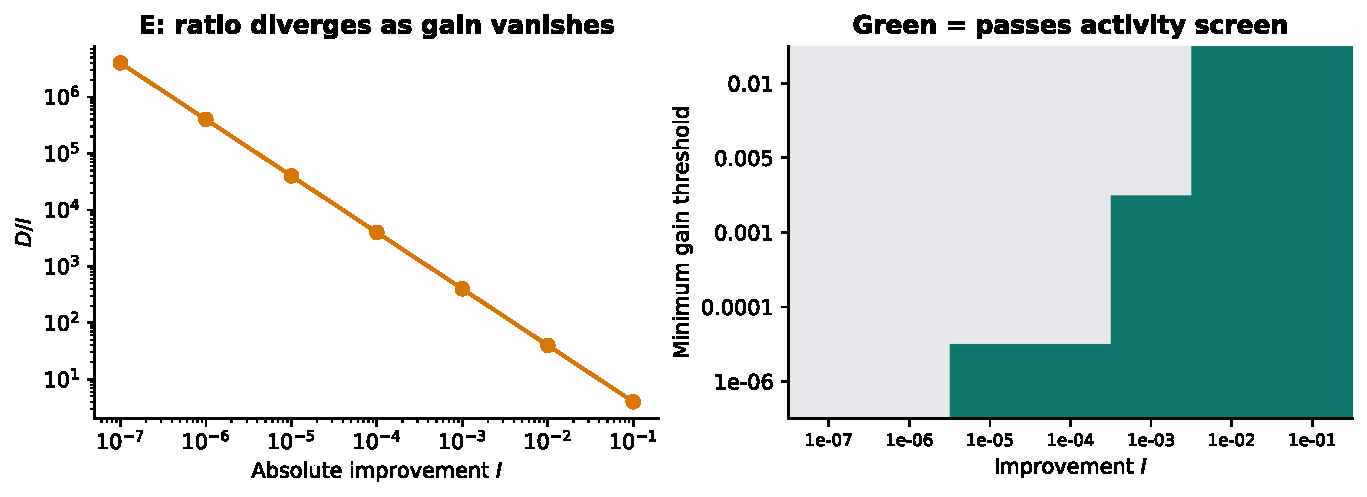
\includegraphics[width=0.96\linewidth]{case_E.pdf}
\caption{A larger exit ratio can accompany a smaller absolute improvement.}\label{fig:E}\end{figure}

Negative controls bound the interpretation of a knee claim.
The linear-front control makes TAFR abstain under the tested configuration.
A nonconvex piecewise-linear front contains an unsupported interior kink that weighted sums cannot select; AWT reaches that row.
Here AWT minimizes $\max_i w_i y_i+10^{-3}w^\top y$ in frozen normalized coordinates.
Reaching the kink does not guarantee that it passes the exit screen, so we record reachability separately.
Twenty permutations of the plateau table preserve its selected compromise under the canonical tie rule.

\section{SNEE needs versioned runtime adapters}\label{sec:snee}
SNEE searches a maximal-change function (MCF) derived from Pareto sensitivity~\cite{snee}.
Its smooth scalarized formulation requires first- and second-order derivatives or approximations.
We pin the authors' code at \texttt{c3464e66} and identify the paper separately as arXiv version 3, revised 19 March 2026.
The code checkpoint predates that version, so executing the checkpoint does not establish parity with every paper table.
The wrapper skips full-front plotting and subfront diagnostics that do not feed back into knee search.

The original-start experiment contains nine problems, two outer optimizers, and three runtime variants.
The optimizers are Nelder--Mead (NM) and the DIRECT partition-based search method.
Variants retain published objective scales, adapt constrained gradient shapes for SciPy, or additionally normalize objectives using frozen payoff bounds.
The corrected adapter completes 45 of 54 jobs and retains nine failures: eight unmodified constrained jobs and the published-scale compatible DIRECT run on VFM1constr.
These failures identify runtime or implementation limits; they do not establish mathematical inapplicability.

Independent inspection corrected our own adapter error before the main comparison.
The first compatibility wrapper flattened gradients globally, including a multiplier calculation that needs a column vector.
Version 2 flattens only one-dimensional decision inputs supplied by the constrained optimizer.
Both batches remain in history; all main summaries use version 2.
A finite-difference check also exposes upstream GRV2 Hessian broadcasting for column inputs; the published-code variants retain that expression.
\begin{table}[htbp]\centering\small\begin{tabular}{lllr}
\toprule
Problem & Published-scale MCF & Normalized MCF & Runs per variant \\
\midrule
DAS1 & 1.0000 [1.0000, 1.0000] & 1.0000 [1.0000, 1.5665] & 30 \\
DO2DK & 1.0000 [1.0000, 1.0000] & 1.0000 [1.0000, 1.0000] & 30 \\
DO2DKtight & 1.0000 [1.0000, 1.0000] & 1.0000 [1.0000, 1.0000] & 30 \\
GRV1 & 1.1820 [1.1820, 1.1820] & 1.1936 [1.1935, 2.1479] & 30 \\
GRV2 & 1.0000 [1.0000, 1.0000] & 1.0000 [1.0000, 1.0000] & 30 \\
VFM1 & 1.4142 [1.4142, 1.4142] & 1.0000 [1.0000, 1.0001] & 30 \\
VFM1constr & 1.4142 [1.3793, 1.5064] & 1.0000 [1.0000, 1.0001] & 30 \\
ZLT1 & 1.0000 [1.0000, 1.0001] & 1.0000 [1.0000, 1.0001] & 30 \\
ZLT1q & 1.0001 [1.0001, 1.0026] & 1.0001 [1.0001, 1.0026] & 30 \\
\bottomrule
\end{tabular}

\caption{MCF median [Q1, Q3] over 30 paired starts. Each scale convention defines its own MCF.}\label{tab:snee}\end{table}

The corrected multi-start experiment uses NM only and completes 540 jobs across nine problems, 30 starts, and two scale conventions. DIRECT appears in the original-start experiment.
Table~\ref{tab:snee} shows that scale conventions affect both values and spread across starts.
A separate 17-candidate TAFR pilot uses the same objective definitions and analytic lower-level solutions for quadratic cases; it returns points on eight of nine problems.
Only symmetric ZLT1, ZLT1q, and GRV2 receive analytic equal-weight targets in this release.
Different budgets and unresolved derivative diagnostics prevent an equal-budget superiority claim.
Dimensional checks cover ZLT1q at $q=3,5,8,10$ and GRV2 at $n=2,10,50,100$, but only validate stationary equal-weight solutions.

\section{PMOP isolates the selection criterion}\label{sec:pmop}
PMOP varies knee geometry and optimization difficulty and supplies knee-specific metrics~\cite{pmop,pmopcode}.
We pin repository \texttt{4fb56cea} and load official true-knee and knee-region arrays.
The common finite table combines 512 Sobol position draws, shape boundaries, every supplied knee, and up to 128 knee-region rows, then removes dominated rows.
All methods receive that table, including exact reference knees.
This construction isolates selection criteria and cannot support a claim about avoiding front generation.
The Python front mapping has formula and boundary checks; numerical parity against a MATLAB runtime remains pending.

Payoff ties expose normalization failures before knee comparison.
Of 42 configurations spanning PMOP1 through PMOP14 and three, five, or eight objectives, 33 produce a zero objective range under the canonical tie rule.
All 42 payoff anchor sets are affinely dependent, so their minimum-norm convex-hull-of-individual-minima (CHIM) scores do not define the intended baseline.
We retain those scores as raw diagnostics and mark CHIM unavailable in main analysis.
A separate oracle-table normalization variant supplies frozen minima and maxima from the common table and completes all configurations.
It uses additional front information and leaves the production estimator unchanged.
For a returned normalized vector $\hat y$, knee error is $d_K=\min_{k\in K^\star}\|\hat y-k\|_2$, with both vectors using these same frozen table bounds.
Success@0.025 counts a configuration when the method returns a point with $d_K\le0.025$; abstention counts as unsuccessful.
\begin{table}[htbp]\centering\small\begin{tabular}{llll}
\toprule
Method & Returned & Error median [Q1, Q3] & Success@0.025 \\
\midrule
TAFR gain variant & 36/42 & 0.0234 [0.0000, 0.2124] & 18/42 \\
Equal normalized weights & 42/42 & 0.0000 [0.0000, 0.1861] & 26/42 \\
TPE-2024-grid & 42/42 & 0.1760 [0.0000, 0.5876] & 17/42 \\
\bottomrule
\end{tabular}

\caption{One-seed PMOP pilot with 17 candidate weights. Error quantiles condition on a returned point; success denominators include all 42 configurations.}\label{tab:pmop}\end{table}

Equal normalized weights outperform the TAFR gain variant on Success@0.025 in this pilot.
Table~\ref{tab:pmop} reports 26 successes for equal weights and 18 for TAFR, which returns a point in 36 configurations.
The table includes exact knees, and default PMOP geometries contain symmetries that equal weights can exploit.
These observations reject a broad accuracy-superiority claim for the present configuration.
Reporting abstention separately prevents conditional error from concealing missing outputs.

Every reference knee receives a support test against the finite feasible table.
Processed records separate all-knee and supported-knee metrics; finite-table support need not imply continuous-front support.
Metrics include nearest-knee error, three success thresholds, knee dissimilarity (KD), knee generational distance (KGD), knee inverted generational distance (KIGD), and one-to-one Hungarian matching.
The MATLAB KGD code uses the norm of nearest distances divided by prediction count; the paper's mean-distance convention differs for multiple predictions.
We preserve both conventions, although this single-point pilot does not evaluate multi-knee discovery.

The exact oracle validates every returned TAFR point in this track.
One of 36 reports understates displacement beyond $10^{-7}$: PMOP12 with five objectives reports about $0.07159$, while the oracle gives about $0.07359$.
Figure~\ref{fig:validity} separates exact finite-table validation from independent continuous samples.
The code provides Friedman and Holm-corrected paired Wilcoxon calculations, but the heterogeneous one-seed pilot supports exploratory diagnostics only.
A final significance claim requires the paired protocol and method-budget controls.
\begin{figure}[htbp]\centering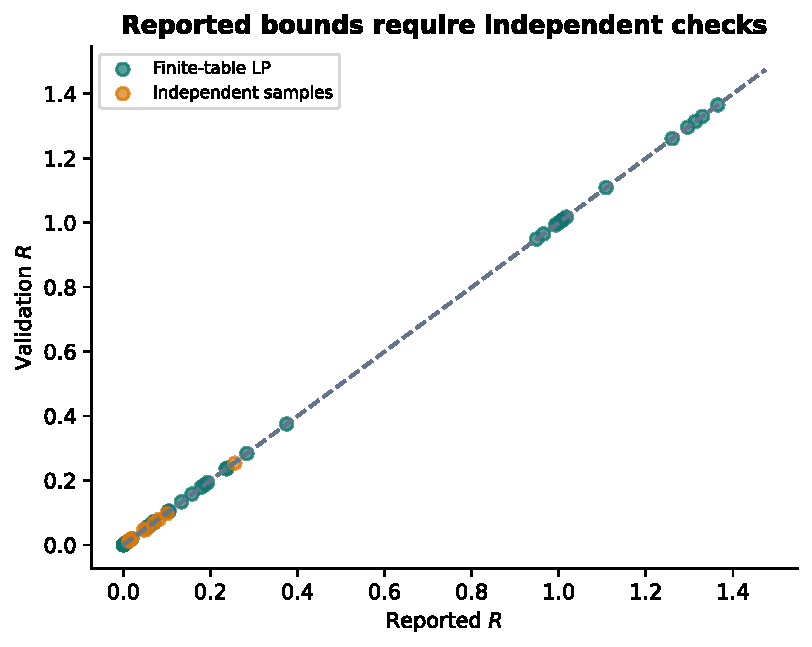
\includegraphics[width=0.60\linewidth]{audit_validity.pdf}
\caption{Independent validation can exceed reported optimizer-map displacement.}\label{fig:validity}\end{figure}

\section{Persistence differs from severity}
Mavrotas and coauthors analyze weight robustness through expanding relative neighborhoods and solution persistence~\cite{mavrotas}.
Our Mavrotas-style diagnostic jointly samples the relative box intersected with the simplex and computes the normalized trapezoidal area under the persistence curve, RI.
The relative neighborhood is $\{u\in\Delta_m:|u_i-w_i|\le\alpha w_i\}$. The pilot integrates over $\alpha=0,0.2,\ldots,1$, using 32 draws at each level for post-analysis of TAFR points and 256 for the portfolio AWT diagnostic.
Rejection sampling in $m-1$ coordinates preserves uniform sampling on that intersection.
The continuous diagnostic declares persistence when normalized objective displacement does not exceed $10^{-3}$, an explicit experimental tolerance.
The diagnostic remains post-analysis of a selected point; ranking candidate weights by RI requires a separate search extension.

Three project-portfolio instances demonstrate the finite discrete workflow.
Each enumerates all $2^{15}$ binary portfolios, applies a capacity constraint, and constructs a nondominated three-objective table.
TAFR returns a point with exact displacement zero at radius $0.05$ in each instance.
Table~\ref{tab:discrete} also reports the equal-weight AWT persistence diagnostic.
Zero displacement on a plateau does not establish the best trade-off geometry or greatest RI; direct TAFR-AWT search remains pending.
\begin{table}[htbp]\centering\small\resizebox{\linewidth}{!}{\begin{tabular}{rrrrrr}
\toprule
Seed & Feasible portfolios & TAFR selected & Exact R & Exit ratio & AWT equal-weight RI \\
\midrule
0 & 8633 & True & 0.0000 & 1.0858 & 0.5531 \\
1 & 8155 & True & 0.0000 & 1.6927 & 0.6172 \\
2 & 8566 & True & 0.0000 & 1.0621 & 0.3980 \\
\bottomrule
\end{tabular}
}
\caption{Exact portfolio pilot and a separately defined AWT persistence diagnostic.}\label{tab:discrete}\end{table}

\section{Dimension changes the audit domain}
A resolution-$H$ lattice contains $\binom{H+m-1}{m-1}$ candidates.
For an interior symmetric clipped neighborhood, the complete vertex count is
\[
 |V_m|=\begin{cases}\binom{m}{m/2},&m\text{ even},\\
 m\binom{m-1}{(m-1)/2},&m\text{ odd}.\end{cases}
\]
The geometry pilot verifies counts through ten objectives by enumeration and reports larger counts analytically.
Figure~\ref{fig:scaling} also measures the closest Sobol candidate to a symmetric quadratic knee over 30 seeds and budgets from 250 to 10,000.
That coverage curve excludes injected equal weights and does not measure full TAFR selection quality.
\begin{figure}[htbp]\centering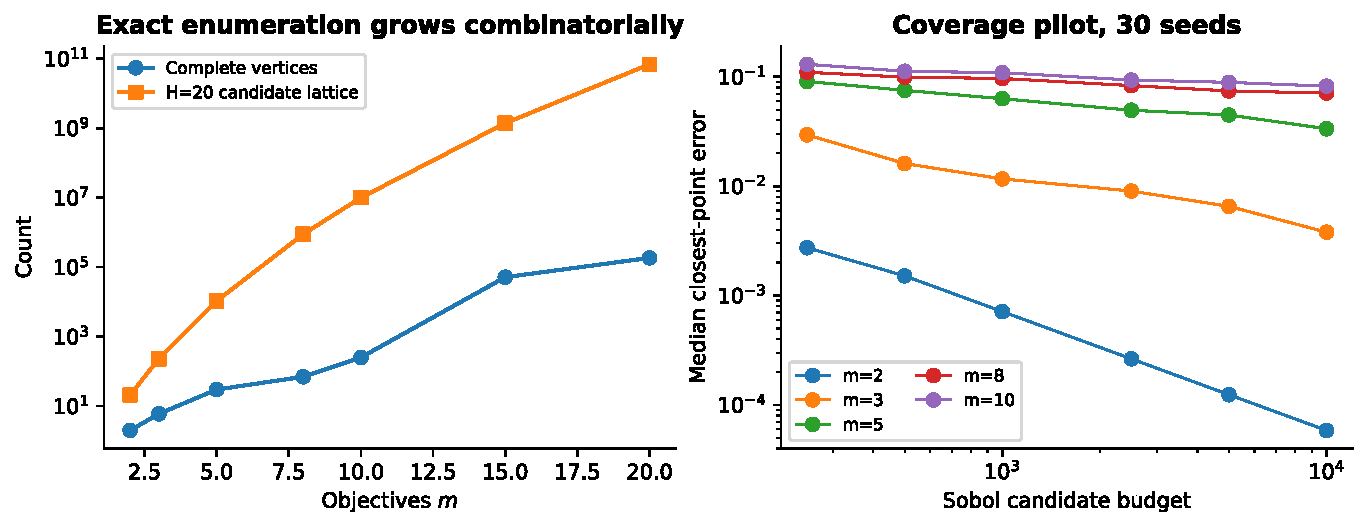
\includegraphics[width=0.96\linewidth]{scalability.pdf}
\caption{Counts grow rapidly; candidate coverage alone does not establish method efficiency.}\label{fig:scaling}\end{figure}

Grouping can hide original-space displacement.
For the four-objective counterexample, averaging groups $(1,3)$ and $(2,4)$ makes $Q$ worse than $P$ in both reduced objectives, so the reduced audit reports zero.
The original domain still contains the switch to $Q$ with displacement $\RfullC$.
Correct grouping retains the trade-off, but the two-dimensional distance has different units from the original distance.
Reduced-space search therefore needs an audit in the original frozen normalized objectives and original perturbation domain.
The example tests hidden deterioration, not a reduction algorithm's speedup.

Equal $L_\infty$ radii allow different total weight movement across dimensions.
The pilot records $\rho_m=0.2/m$ and maximum total-variation distance, defined as half the $L_1$ weight difference.
A final comparison should add fixed total-variation and fixed-radius conditions separately.
Production radius bisection also resamples at each radius, which can make estimated displacement nonmonotone.
Nested samples restore monotonicity of the sampled estimate but do not prove exact stability. An exact stability claim needs a global oracle or a verified adversarial solver.

\section{Ammonia exposes objective dependence}\label{sec:ammonia}
The scheduling pilot uses the existing public model and datasets at commit \texttt{8a5e9869}~\cite{ammoniacode}.
Its objectives are operating cost, emissions, water use, and an electrolyzer-throughput safety proxy over 48 hours.
The Python port preserves material balances, integer electrolyzer counts, ammonia ramp timing, terminal inventories, and the 45,000 kg minimum ammonia target.
HiGHS solves each mixed-integer linear program with relative gap $10^{-3}$ and a ten-second limit.
Records include solver status, gap, and constraint residual; forecasts remain fixed.

The input manifest contains 12 stratified windows, of which this release runs two.
Inputs use USD/kWh for electricity prices and kgCO$_2$/kWh for carbon intensity.
Strata use temporal price-carbon Pearson correlation as a proxy, which differs from objective correlation across feasible schedules.
Executed cases are CAISO/LA January 2022 at source row 624 and ISO-NE 2022 at row 5904.
We retain source-row identifiers without inferring timestamps absent from the feature files.

The primary payoff-normalized pilot abstains in both windows.
ISO-NE water and safety anchor ranges lie near machine precision, making normalized displacement numerically unstable.
The separate global-bound diagnostic minimizes and maximizes each objective, expands candidates from five to 17, and increases radius bisections from three to six.
It changes both bounds and search budget, so it cannot isolate normalization's causal effect.
It returns a LA point and still abstains for ISO-NE.
\begin{table}[htbp]\centering\scriptsize\resizebox{\linewidth}{!}{\begin{tabular}{llrrrrr}
\toprule
Case & Method & Cost & CO2 & Water & Safety & Validation R \\
\midrule
LA/Payoff & TAFR & NA & NA & NA & NA & NA \\
LA/Payoff & Equal & 2.85e+04 & 1.3e+05 & 4.99e+04 & 94.3 & 0.532 \\
LA/Payoff & TPE & 3.23e+04 & 1.12e+05 & 4.99e+04 & 94.3 & 0.116 \\
NE/Payoff & TAFR & NA & NA & NA & NA & NA \\
NE/Payoff & Equal & 4.53e+04 & 1.23e+05 & 4.99e+04 & 94.3 & 0 \\
NE/Payoff & TPE & 3.8e+04 & 1.16e+05 & 4.99e+04 & 94.3 & 14.5 \\
LA/Global & TAFR & 3.11e+04 & 1.13e+05 & 4.99e+04 & 94.3 & 0.0172 \\
LA/Global & Equal & 3.09e+04 & 1.15e+05 & 4.99e+04 & 94.3 & 0.157 \\
LA/Global & TPE & 3.17e+04 & 1.12e+05 & 4.99e+04 & 94.3 & 0.0246 \\
NE/Global & TAFR & NA & NA & NA & NA & NA \\
NE/Global & Equal & 3.77e+04 & 1.16e+05 & 4.99e+04 & 94.3 & 0.00738 \\
NE/Global & TPE & 3.76e+04 & 1.17e+05 & 4.99e+04 & 94.3 & 0.000712 \\
\bottomrule
\end{tabular}
}
\caption{Actual 48-hour schedules. NA marks abstention. Cost uses USD, CO2 uses kg, water follows source volume coefficients, and safety is a throughput index. Each bound convention defines its own normalized validation $R$.}\label{tab:ammonia}\end{table}

The LA global-bound point trades cost against emissions while keeping water and safety at their minima.
Independent sampled displacement is about $0.01716$, matching reported displacement, with exit ratio about $1.508$.
Its radius estimate is zero at the diagnostic's bisection resolution, so the result does not establish a positive exact plateau radius.
Validation uses at least 256 new perturbations; a finite sample cannot prove the continuous maximum.
These observations support a decision diagnostic, not a general four-way knee claim.

The objectives explain the weak four-way interpretation.
Let $H$ denote total electrolytic hydrogen and $B$ total purchased hydrogen.
The model imposes only a lower bound on ammonia output, and every retained schedule attains 45,000 kg. On this fixed-output slice, terminal inventories fix $H+B$; water equals $9H+4.5B$ and safety equals $H/33.3$.
Water and safety therefore depend affinely on the same scalar $H$.
The source declares additional risk constants but does not include them in this objective; we do not silently add startup or storage risk.
A distinct safety objective needs a separately justified model variant.

\section{The article should follow the evidence}\label{sec:outline}
A draft for the European Journal of Operational Research (EJOR) fits the evidence through preference analysis, exact weight cells, and solver-based decision support.
Mavrotas-style persistence is the closest conceptual comparison and belongs in the main related-work table.
The research direction is direct preference search with severity and exit checks, followed by independent auditing.
The present results do not establish universal recovery, continuous global certification, or overall PMOP superiority.
A submission to IEEE Transactions on Cybernetics (TCYB) additionally needs population comparisons and full search-efficiency results.
\begin{enumerate}
\item \textbf{Decision problem.} Explain non-extreme compromises under bounded preference changes. Keep the proposed direct-search claim conditional on remaining gates.
\item \textbf{Finite-radius formulation.} Define normalization, the optimizer map, severity, stability, absolute gains, and abstention, including tie and solver-accuracy assumptions.
\item \textbf{Mechanisms and limits.} Present exact cells, the missing four-objective perturbation, the interior-cell construction, and the vanishing-gain failure.
\item \textbf{Algorithm and variants.} Describe candidate search, perturbation geometry, gain thresholds, and original-space validation after reduction. Distinguish screening from exact certification.
\item \textbf{Controlled evaluation.} Reproduce versioned SNEE, separate PMOP selection from full-decision optimization, and distinguish supported from unsupported knees.
\item \textbf{Discrete and scheduling decisions.} Compare weighted sums with AWT, severity with persistence, and the physical decisions behind selected schedules.
\item \textbf{Limits and guidance.} Report abstentions, normalization sensitivity, derivative discrepancies, solver failures, and budgets.
\end{enumerate}

Four gates determine the next release.
First, freeze a justified absolute-gain rule and alternate-optimum normalization policy as named variants.
Second, validate the PMOP port numerically and implement the full-decision track with a reference vector guided evolutionary algorithm (RVEA), knee-selection rules, a knee point driven evolutionary algorithm (KnEA), and a valid geometric baseline. The pinned PlatEMO platform supplies these population algorithms~\cite{platemo}.
Third, run paired 30-seed equal-budget comparisons, direct AWT and RI-search extensions, and the full ablation matrix.
Fourth, justify the scheduling safety objective and expand to the 12-window manifest.
The completed counterexamples provide acceptance tests for those changes.

\appendix\section{Versions and reproduction}
The branch is \texttt{experiments/common-core-v1}.
Pinned sources are SNEE \texttt{c3464e66}, PMOP \texttt{4fb56cea}, and ammonia \texttt{8a5e9869}.
The runtime uses Python 3.12.13, NumPy 2.3.5, SciPy 1.17.0, and bundled HiGHS 1.8.0 on Linux with an AMD EPYC 9V74 host CPU.
Per-bundle metadata records environment and seeds; an explicit ledger corrects early execution-start revisions recorded at serialization.
New runs freeze source hashes at import.
\begin{verbatim}
git submodule update --init --recursive
python -m pip install -e . -r experiments/requirements.txt
PYTHONPATH=src python -m experiments.runners.run_experiment smoke
PYTHONPATH=src python -m experiments.runners.run_experiment adversarial
PYTHONPATH=src python -m experiments.runners.run_experiment snee
PYTHONPATH=src python -m experiments.runners.run_experiment pmop
PYTHONPATH=src python -m experiments.runners.run_experiment scalability
PYTHONPATH=src python -m experiments.runners.run_experiment ammonia
PYTHONPATH=src python -m experiments.runners.run_experiment report
cd experiments/note
latexmk -pdf TAFR_Experiment_Note.tex
\end{verbatim}
Drivers checkpoint completed jobs and retain failures.
Adapter changes require new versioned output directories to avoid reusing old measurements.
Artifacts include raw JSON, YAML configurations, processed CSV, vector figures, LaTeX tables, execution status, and a claim ledger.
Null counters denote uncollected measurements, including peak memory and some baseline call counts; they never denote measured zero cost.

\begin{thebibliography}{9}
\bibitem{proposal} H. Wang.
\emph{Novel Algorithms for the Efficient Solution of Many-Objective Optimization Problems}.
Thesis Proposal Exam Written Proposal, University of Michigan, 22 May 2024.
User-supplied project document; this release excludes the source PDF and CV.
\bibitem{platemo} Y. Tian, R. Cheng, X. Zhang, and Y. Jin.
PlatEMO: A MATLAB platform for evolutionary multi-objective optimization.
IEEE Computational Intelligence Magazine, 12(4):73--87, 2017.
\bibitem{snee} T. Giovannelli, M. M. Raimundo, and L. N. Vicente.
\emph{Pareto sensitivity, most-changing sub-fronts, and knee solutions}.
arXiv:2501.16993v3, 2026. \url{https://arxiv.org/abs/2501.16993v3}.
Code: \url{https://github.com/tommaso-giovannelli/snee}.
\bibitem{pmop} G. Yu, Y. Jin, and M. Olhofer.
\emph{Benchmark Problems and Performance Indicators for Search of Knee Points in Multiobjective Optimization}.
IEEE Transactions on Cybernetics, 50(8), 2020.
\href{https://doi.org/10.1109/TCYB.2019.2894664}{doi:10.1109/TCYB.2019.2894664}.
\bibitem{pmopcode} G. Yu. PMOPs-Benchmark, pinned source and reference data.
\url{https://github.com/GYResearch/PMOPs-Benchmark}.
\bibitem{mavrotas} G. Mavrotas, O. Pechak, E. Siskos, H. Doukas, and J. Psarras.
\emph{Robustness analysis in Multi-Objective Mathematical Programming using Monte Carlo simulation}.
European Journal of Operational Research, 240(1):193--201, 2015.
\href{https://doi.org/10.1016/j.ejor.2014.06.039}{doi:10.1016/j.ejor.2014.06.039}.
\bibitem{ammoniacode} Project scheduling model and datasets.
\url{https://github.com/beam4869/ML_scheduling}.
\end{thebibliography}\end{document}
